\section{Results}
\label{sec:result}

The pipeline retains 490,911 valid traceroutes from 707,314 raw records and
produces 3,291,063 atomic segments. Of 2,432,559 mappable segments, 555,119
reach candidate landing points, 171,232 satisfy the corridor constraints, and
124,350 support at least one feasible inter-region corridor. The 370 auditable
country--measurement units contain 222 DNS Root, 53 application, and 95
topology-reference units.

\subsection{Inter-Region Candidate Exposure}
\label{subsec:overall-exposure}

Inter-region candidates occur infrequently for most service-facing
populations. Pooling eligible Root observations within each country by valid-
trace count yields median DNS exposure of 5.50\% (IQR 1.10--23.04\%; mean
17.80\%). Median country--measurement exposure is 1.90\% for Wikipedia,
1.96\% for Reddit, and 1.43\% for Netflix Assets. The two dynamic multi-
target references reach 23.24\% for MSM~5051 and 23.81\% for MSM~5151.

Country-matched comparisons retain source country but change the target
population. DNS exposure is lower than MSM~5051 in 70 of 77 shared countries,
with a median paired difference of (-14.52) percentage points. It is lower
than MSM~5151 in 54 of 59 shared countries, with a median difference of
(-14.82) points. These comparisons describe the measured populations; they
do not identify a deployment or target-selection effect.

\begin{figure*}[t]
  \centering
  \subfloat[Country--measurement exposure.\label{fig:result-overview-distribution}]{%
    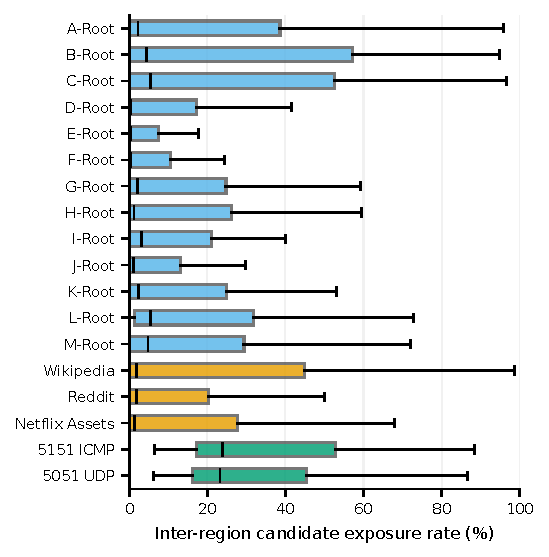
\includegraphics[width=0.39\textwidth]{figures/fig_result_overview_distribution.pdf}}
  \hspace{0.045\textwidth}
  \subfloat[Country-matched comparison.\label{fig:result-overview-paired}]{%
    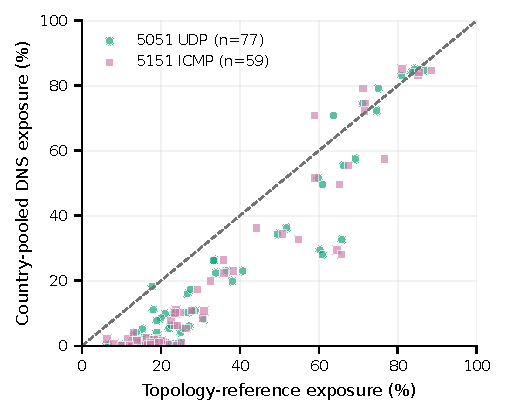
\includegraphics[width=0.34\textwidth]{figures/fig_result_overview_paired.pdf}}
  \caption{Inter-region candidate exposure in the observed measurement
  populations.}
  \label{fig:result-overview}
\end{figure*}

\subsection{Layer Agreement within Measurement Families}
\label{subsec:family-agreement}

Pooling all 370 units gives a rank association of 0.47 between network and
corridor Top-2 shares. This pooled coefficient includes the separation between
measurement families and does not isolate the within-family relationship.

Table~\ref{tab:family-agreement} reports Layer Agreement within each family
under the three existing allocation rules. Projection-score weighting gives
0.176 for 219 DNS units, 0.229 for 53 application units, and 0.012 for 95
topology-reference units. The coefficients describe the ordering of units
within each family.

\begin{table}[t]
  \centering
  \caption{Layer Agreement by measurement family.}
  \label{tab:family-agreement}
  \footnotesize
  \setlength{\tabcolsep}{4.0pt}
  \begin{tabular}{lrrrr}
    \toprule
    Family & (n) & Equal & Score & Top-1 \\
    \midrule
    DNS Roots & 219 & 0.096 & 0.176 & 0.330 \\
    Applications & 53 & 0.030 & 0.229 & 0.372 \\
    Topology references & 95 & 0.139 & 0.012 & 0.122 \\
    \bottomrule
  \end{tabular}
\end{table}

The equal-share primary outputs also show different absolute corridor breadth
across the observed families. Median corridor Top-2 share is 72.0\% for DNS,
70.3\% for applications, and 30.6\% for topology references; median effective
corridor counts are 3.84, 3.51, and 18.01. Because the target populations
differ, these levels are descriptive family summaries rather than a controlled
estimate of a service effect.

\subsection{Layer Agreement Differs by Geography}
\label{subsec:geographic-agreement}

The geographic split separates service-facing populations that are combined in
the family-level summaries. Under projection-score weighting, Layer Agreement
is 0.632 across 67 island and archipelagic units and 0.001 across 202 coastal-
mainland units. The observed difference is 0.631. Landlocked service-facing
units are not members of either geographic group in this comparison.

\begin{table}[t]
  \centering
  \caption{Service-facing Layer Agreement by geography and allocation rule.}
  \label{tab:geographic-agreement}
  \footnotesize
  \setlength{\tabcolsep}{3.5pt}
  \begin{tabular}{lrrr}
    \toprule
    Allocation & Island/arch. & Coastal mainland & Difference \\
    \midrule
    Equal share & 0.380 & -0.081 & 0.461 \\
    Projection score & 0.632 & 0.001 & 0.631 \\
    Top-1 & 0.820 & 0.105 & 0.715 \\
    \bottomrule
  \end{tabular}
\end{table}

The geographic difference remains in the same direction under all three
allocation rules. The association increases as the allocation places more mass
on higher-scoring corridors. These results record sensitivity to candidate
allocation; without physical-route ground truth, they do not establish that
one allocation recovers the true association.

\subsection{Exposure and Conditional Breadth}
\label{subsec:geography}

Geography also separates exposure from conditional corridor breadth in the
equal-share outputs. Island and archipelagic countries have median pooled DNS
exposure of 49.61\% across 9 countries, compared with 7.88\% for 54 other
coastal countries and 1.70\% for 14 landlocked countries.

Conditional breadth follows a different ordering. Island and archipelagic
countries have median corridor Top-2 share of 53.3\% and 5.58 effective
corridors. Other coastal countries reach 75.4\% and 3.39. The two represented
landlocked countries reach 80.2\% and 2.51. Across 38 countries with both
pooled exposure and an auditable corridor summary, exposure has Spearman
association (-0.29) with corridor Top-2 share and 0.30 with effective
corridor count.

\begin{figure*}[t]
  \centering
  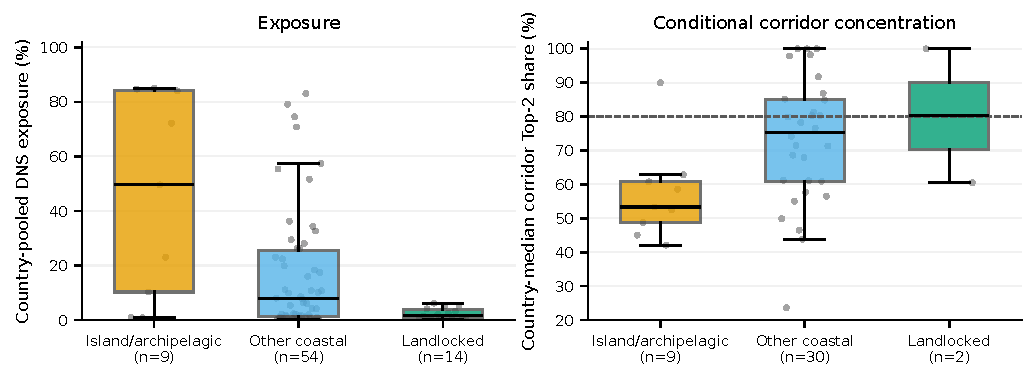
\includegraphics[width=0.72\textwidth]{figures/fig_country_geography_30km.pdf}
  \caption{DNS exposure and equal-share corridor concentration by geography.}
  \label{fig:country-geography}
\end{figure*}

\subsection{Contraction Is Not the Only Outcome}
\label{subsec:heterogeneity}

Using the paper's descriptive 80\% Top-2 threshold, 81 of 275 service-facing
units (29.5\%) are network-broad/corridor-concentrated and 158 (57.5\%) remain
broad at both layers. Eighteen (6.5\%) are concentrated at both layers, and 18
(6.5\%) are network-concentrated/corridor-broad. Four of 95 topology-reference
units (4.2\%) enter the contraction class; the other 91 remain broad at both
layers.

Continuous measures show changes within the threshold classes. Corridor Top-2
share increases in 184 of 275 service-facing units (66.9\%), and effective
category count contracts in 204 (74.2\%). Of 239 units with a broad network
distribution, 178 (74.5\%) move upward in Top-2 share: 81 cross the threshold,
while 97 remain broad at both layers with a median increase of 6.3 percentage
points.

\begin{figure*}[t]
  \centering
  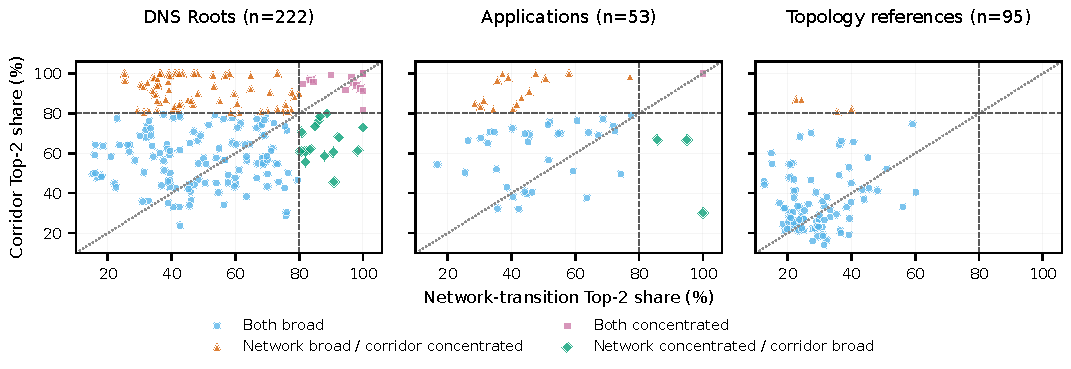
\includegraphics[width=0.92\textwidth]{figures/fig_cross_layer_distribution.pdf}
  \caption{Equal-share network-transition and corridor Top-2 shares for the
  370 auditable units. The 80\% lines define the descriptive classes.}
  \label{fig:cross-layer}
\end{figure*}

Three existing cases show different outcomes. \textbf{Singapore--Netflix}
moves from 32.5\% network Top-2 share to 65.0\% corridor Top-2 share, while
its effective count contracts from 19.86 to 3.41. It narrows without crossing
the 80\% threshold. \textbf{New Zealand--Netflix} moves from 63.6\% to
37.6\%, with effective count expanding from 5.18 to 6.92.
\textbf{Singapore--H-Root} moves from 39.6\% to 50.1\%, and its effective
count contracts from 20.67 to 5.99 while normalized entropy changes only
slightly. Bounded multi-corridor segments account for 99.9\%, 78.1\%, and
98.2\% of candidate-bearing observations in these cases, respectively.
